\chapter{Arhitektura i dizajn sustava}
		
Da bismo razradili arhitekturu web aplikacije za poboljšanje dostupnosti knjiga prevedenih na hrvatski i srodne jezike, detaljnije ćemo opisati njene komponente, organizaciju i međusobnu komunikaciju. Evo ključnih elemenata:
	\\

        \textbf{1. Stil Arhitekture}\\
        Stil arhitekture bi mogao biti mikroservisni ili slojeviti (npr. MVC - Model-View-Controller). Mikroservisni pristup omogućava modularnost i lako skaliranje, dok slojeviti pristup olakšava razvoj i održavanje. Prilikom razvoja naše aplikacije odabran je MVC model.
        \\
        
        \textbf{2. Podsustavi}\\

        Podsustavi se mogu podijeliti na:
        \begin{itemize}
		  \item {Korisničko sučelje (UI): Front-end komponenta zadužena za interakciju s korisnicima.}
		  \item {Poslovna logika: Središnji dio koji upravlja funkcionalnostima aplikacije.}
		  \item {Baza podataka: Spremište podataka gdje se čuvaju informacije o knjigama, korisnicima, ponuditeljima, itd.}		
            \item {Autentikacija i autorizacija: Sustav za upravljanje korisničkim pristupima i ovlastima.}	
             \item {Integracija vanjskih usluga: Za funkcionalnosti poput prikaza karte (npr. integracija OpenStreetMap).}		
	   \end{itemize}

        \textbf{3. Preslikavanje na Radnu Platformu}\\

        Komponente se raspoređuju na servere i klijentske uređaje:
        \begin{itemize}
		  \item {Server: Hostira poslovnu logiku, bazu podataka, autentikaciju i API za integraciju vanjskih usluga.}
		  \item {Klijent: Uređaji korisnika (mobiteli, tableti, računala) s web preglednikom za pristup UI.}
	   \end{itemize}
    
    \textbf{4. Spremišta Podataka}\\

        Centralizirana baza podataka (SQL ili NoSQL) koja pohranjuje:
        \begin{itemize}
		  \item {Podatke o knjigama.}
		  \item {Informacije o korisnicima i ponuditeljima.}
		  \item {Zahtjeve za prijevod i ponude.}				
	   \end{itemize}

    \textbf{5. Mrežni Protokoli}\\
    
    \begin{itemize}
		  \item {HTTP/HTTPS: Za komunikaciju između klijenta i servera.}
		  \item {API protokoli (REST, GraphQL): Za upite i manipulaciju podacima.}
	   \end{itemize}

    \textbf{6. Globalni Upravljački Toke}\\

        Sustav bi koristio zahtjev-odgovor model za komunikaciju između klijenta i servera. Autentikacija i autorizacija korisnika odvijaju se na početku sesije.
    
    \textbf{7. Sklopovsko-Programski Zahtjevi}\\

    \begin{itemize}
		  \item {Server: Pouzdan i skalabilan, s dovoljno resursa za obradu zahtjeva i pohranu podataka.}
		  \item {Klijent: Kompatibilnost s modernim web preglednicima i prilagodljivost različitim veličinama ekrana.}			
	   \end{itemize}
	   
	   
	   \begin{itemize}
	   	\item {Prikazuje raspored glavnih komponenti: UI, poslovna logika, baza podataka, autentikacija.}
	   	\item {Ilustrira komunikaciju između klijenta i servera.}			
	   \end{itemize}
	   
		
		\eject
		
		\begin{figure}[H]
			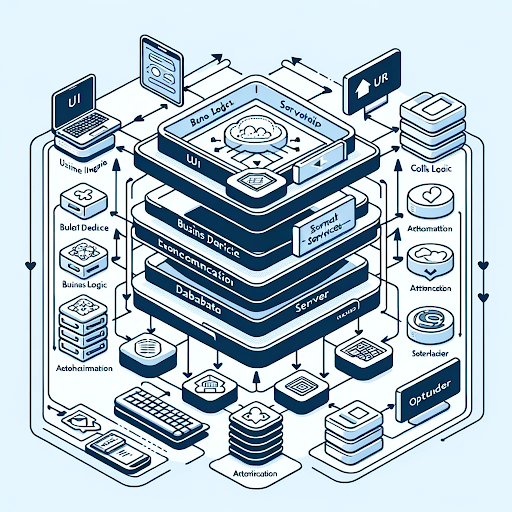
\includegraphics[width=\textwidth]{slike/arhitektura.PNG} %veličina u odnosu na širinu linije
			\centering
			\caption{Osnova arhitekture}
			\label{fig5:promjene}
		\end{figure}
		
		\eject
	
  Skica ilustrira sljedeće komponente i njihovu međusobnu komunikaciju:
   \begin{itemize}
		  \item {Korisničko sučelje (UI): Na klijentskim uređajima (mobitel, tablet, računalo).}
		  \item {Poslovna logika: Dio koji se nalazi na serveru.}	
            \item {Baza podataka: Spremište podataka također na serveru.}
		  \item {Autentikacija: Dio za upravljanje korisničkim pristupom.}	
            \item {Integracija vanjskih usluga: Na primjer, OpenStreetMap za prikaz karata.}
	   \end{itemize}

Izbor Model-View-Controller (MVC) arhitekture za ovu web aplikaciju temelji se na nekoliko ključnih principa oblikovanja koje sam uzimao u obzir:

	\eject

 \textbf{1. Separacija Briga (Separation of Concerns)}\\

MVC arhitektura odlično odvaja različite aspekte aplikacije:
\begin{itemize}
		  \item {Model: Predstavlja podatke i poslovnu logiku aplikacije. U ovom slučaju, model bi upravljao podacima knjiga, korisnika, ponuda i zahtjeva za prijevod.}
		  \item {View: Odnosi se na korisničko sučelje. U našoj aplikaciji, ovo bi bilo mjesto gdje korisnici pretražuju knjige, pregledavaju ponude, i komuniciraju sa sustavom.}	
            \item {Controller: Djeluje kao posrednik između Modela i Viewa, obrađuje korisničke zahtjeve, ažurira model i konačno šalje podatke natrag viewu.}
	   \end{itemize}

Ova jasna podjela pomaže u organizaciji koda, olakšava održavanje i omogućava lakše testiranje pojedinih komponenti.
	\\

 \textbf{2. Skalabilnost i Fleksibilnost}

MVC podržava skalabilnost. Kako se aplikacija razvija, svaki dio (Model, View, Controller) može se neovisno skalirati ili modificirati. Ovo je posebno korisno za aplikacije koje imaju potencijal rasti, kao što je naš slučaj s web platformom za knjige.
	\\

 \textbf{3. Podrška za Više Klijentskih Platformi}

S obzirom na to da se aplikacija mora prilagoditi različitim uređajima (mobilnim telefonima, tabletima, računalima), MVC omogućava razvoj različitih vrsta viewova koji mogu koristiti isti model i controller logiku. To znači da možemo imati različite korisničke sučelja za mobilne uređaje i desktop računala, dok se poslovna logika i obrada podataka ne mijenjaju.
	\\

 \textbf{4. Održavanje i Nadogradnja}

MVC struktura pojednostavljuje ažuriranja i održavanje. Ako trebate promijeniti poslovnu logiku, to se može učiniti u modelu bez utjecaja na view. Slično, izmjene u korisničkom sučelju ne utječu na poslovnu logiku aplikacije.
	\\
	
 \textbf{5. Zajednica i Resursi}

MVC je popularan i dobro dokumentiran arhitekturni obrazac. Postoji obilje resursa, biblioteka i okvira koji podržavaju MVC, što može značajno ubrzati razvoj i pružiti bolju podršku tijekom razvojnog procesa.

Zbog ovih razloga, MVC se čini kao optimalan izbor za arhitekturu ove web aplikacije, pružajući dobru osnovu za jasno strukturiran, održiv i fleksibilan razvoj.


Organizacija sustava za opisanu web aplikaciju s najviše razine apstrakcije može se podijeliti u četiri glavne komponente: klijent-poslužitelj model, baza podataka, datotečni sustav, i grafičko sučelje. Ove komponente zajedno omogućavaju funkcionalnost, skalabilnost i korisničku interakciju potrebnu za uspješan rad aplikacije.

	\eject

 \textbf{1. Klijent-Poslužitelj Model} \\

U klijent-poslužitelj modelu, aplikacija je podijeljena na dva glavna dijela: klijent (front-end) koji se izvodi na korisničkom uređaju i poslužitelj (back-end) koji obrađuje zahtjeve i šalje odgovore.
\begin{itemize}
		  \item {Klijent (Front-end): Koristi web preglednik ili mobilnu aplikaciju za pristup aplikaciji. Odgovoran je za prikupljanje korisničkih ulaza, prikazivanje podataka korisnicima i slanje zahtjeva poslužitelju.}
		  \item {Poslužitelj (Back-end): Hostira aplikaciju, obrađuje zahtjeve, vrši operacije nad bazom podataka, i vraća rezultate klijentu. Također upravlja autentikacijom, autorizacijom, i sigurnošću.}	\\
	   \end{itemize}
	   


 \textbf{2. Baza Podataka}

Baza podataka je središnje mjesto za pohranu svih podataka koji su relevantni za aplikaciju. Uključuje:
\begin{itemize}
		  \item {Podatke o knjigama: Nazive, autore, žanrove, godine izdanja, itd.}
		  \item {Korisničke podatke: Informacije o registriranim i neregistriranim korisnicima.}	
            \item {Ponude i zahtjeve: Informacije o dostupnosti knjiga, ponuditeljima, i zahtjevima za prijevod.} \\
	   \end{itemize} 


 \textbf{3. Datotečni Sustav}

Datotečni sustav se koristi za pohranu i upravljanje datotekama koje nisu direktno povezane s bazom podataka, poput:
\begin{itemize}
		  \item {Slika korica knjiga: Pohranjene kao datoteke koje se mogu prikazivati u korisničkom sučelju.}
		  \item {Dokumenti: Uključujući priručnike, upute za korisnike, i druge dokumente.} \\
	   \end{itemize} 

 \textbf{4. Grafičko Sučelje}

Grafičko sučelje (GUI) je ono što korisnik vidi i s čime interagira. Uključuje:
\begin{itemize}
		  \item {Web stranice: Dizajnirane za jednostavno korištenje i navigaciju, s funkcionalnostima kao što su pretraga, pregled knjiga, i slanje zahtjeva.}
		  \item {Mobilno sučelje: Prilagođeno za manje ekrane i osjetljivo na dodir, s sličnim funkcionalnostima kao web verzija.}	\\
	   \end{itemize} 

Svaka od ovih komponenti igra ključnu ulogu u uspješnom funkcioniranju aplikacije, omogućujući efikasnu obradu podataka, intuitivnu korisničku interakciju i sigurnost informacija.

\eject

Organizacija aplikacije koja koristi Model-View-Controller (MVC) arhitekturu s jasno definiranim frontend i backend slojevima omogućava efikasno upravljanje kodom i funkcionalnostima. Evo kako bi se to moglo strukturirati:

 \textbf{1. Frontend (Klijentska strana)}\\

Frontend je ono što korisnik vidi i s čime interagira. U MVC arhitekturi, to uglavnom obuhvaća "View" komponentu.
\begin{itemize}
		  \item {Tehnologije: HTML, CSS, JavaScript, i frameworki poput React, Angular ili Vue.js.}
		  \item {Zadaće:
    \begin{itemize}
		  \item {Prikaz podataka: Dinamički prikazuje podatke dobivene s backend-a.}
		  \item {Korisničko sučelje: Omogućava interakciju s korisnikom, prikuplja korisničke zahtjeve i šalje ih backend-u.}	
            \item {Odgovor na korisničke akcije: Ažuriranje sučelja na temelju korisničkih interakcija i podataka s backend-a.}
	   \end{itemize}}	
            
	   \end{itemize}


 \textbf{2. Backend (Poslužiteljska strana)}\\

Backend se bavi obradom podataka, poslovnom logikom i interakcijom s bazom podataka. U MVC arhitekturi, to uključuje "Model" i "Controller" komponente.
\begin{itemize}
		  \item {Tehnologije: Server-side jezici poput Node.js, Python (Django, Flask), Ruby on Rails, Java (Spring), itd.}
		  \item { Zadaće:
            \begin{itemize}
		  \item { Controller:
                    \begin{itemize}
		  \item {Upravlja zahtjevima s frontend-a.}
		  \item {Prosljeđuje podatke između View-a i Modela.}	
            \item {Upravlja tokom podataka i obradi zahtjeva.}
	   \end{itemize}}
        \item { Model:
                    \begin{itemize}
		  \item {Predstavlja poslovnu logiku i podatke.}
		  \item {Interakcija s bazom podataka.}	
            \item {Obrada podataka (CRUD operacije - Create, Read, Update, Delete).}
	   \end{itemize}}
	   \end{itemize}}	
	   \end{itemize}


 \textbf{3. Komunikacija između Frontend-a i Backend-a}\\

Komunikacija između frontend-a i backend-a obično se odvija preko API-ja (Application Programming Interface), koristeći HTTP/HTTPS protokole.
\begin{itemize}
		  \item {API (najčešće REST ili GraphQL): Definira kako frontend šalje zahtjeve backend-u i kako backend vraća odgovore.}
		  \item {JSON format: Često korišten format za slanje podataka između frontend-a i backend-a.}	
	   \end{itemize}


 \textbf{4. Baza Podataka}\\

Iako tehnički nije dio MVC strukture, baza podataka je ključna komponenta koja surađuje s Modelom. Ona pohranjuje sve podatke potrebne za aplikaciju.
\begin{itemize}
		  \item {Tehnologije: SQL (MySQL, PostgreSQL) ili NoSQL (MongoDB, Cassandra) baze podataka.}
		  \item {Zadaće: Pohrana i dohvaćanje podataka potrebnih za aplikaciju.}	
	   \end{itemize}

U ovakvoj organizaciji, svaki sloj ima jasno definiranu ulogu, što doprinosi boljem razumijevanju koda, lakšem održavanju i skaliranju aplikacije. Frontend i backend mogu se neovisno razvijati i optimizirati, što pruža fleksibilnost i efikasnost u razvojnom procesu.

\eject

				
		\section{Baza podataka}
		
		
			\subsection{Opis tablica}
				
				
				\begin{longtblr}[
					label=none,
					entry=none
					]{
						width = \textwidth,
						colspec={|X[6,l]|X[6, l]|X[20, l]|}, 
						rowhead = 1,
					} %definicija širine tablice, širine stupaca, poravnanje i broja redaka naslova tablice
					\hline \SetCell[c=3]{c}{\textbf{Knjiga}}	 \\ \hline[3pt]
					\SetCell{LightGreen}ISBN & VARCHAR(13) & \\ \hline
					naslov	& VARCHAR & \\ \hline 
					autori & VARCHAR &   \\ \hline 
					jezik & CHAR(3)	& troslovni kod po ISO 639-1 standardu 	\\ \hline 
					izdavač & VARCHAR & 	\\ \hline
					brojIzdanja & INT & 	\\ \hline 
					godinaIzdanja & INT & 	\\ \hline
					katIzdavača & CHAR(3) & 	\\ \hline
					zahtZaPr & INT & 	\\ \hline
					očuvanost & VARCHAR & 	\\ \hline
					opis & VARCHAR & 	\\ \hline
					slika & BYTEA & 	\\ \hline
					žanr & VARCHAR & 	
					\\
					
					\hline \SetCell[c=3]{c}{\textbf{Knjiga dobavljivost}}	 \\ \hline[3pt]
					\SetCell{LightBlue}ISBN & VARCHAR(13) & \\ \hline
					dobavljivost & CHAR(3) &
					\\
					
					\hline \SetCell[c=3]{c}{\textbf{Ponuditelj}}	 \\ \hline[3pt]
					\SetCell{LightGreen}korisničkoIme & VARCHAR(32) & \\ \hline
					lozinka	& VARCHAR(32) &   	\\ \hline 
					naziv & VARCHAR &   \\ \hline 
					adresa & VARCHAR	&  		\\ \hline 
					epošta & VARCHAR & 	\\ \hline
					telefon & VARCHAR & 	\\ \hline 
					godinaIzdanja & INT & 	\\ \hline
					katIzdavača & CHAR(3) & 	\\ \hline
					zahtZaPr & INT & 	\\ \hline
					lokacija & POINT & 	\\ \hline
					tip & VARCHAR & izdavač, antikvarijat, preprodavač
					\\
					
					\hline \SetCell[c=3]{c}{\textbf{čekaOdobrenje}}	 \\ \hline[3pt]
					\SetCell{LightBlue}korisničkoIme & VARCHAR(32) & \\ \hline
					status & VARCHAR &
					\\
					
					\hline \SetCell[c=3]{c}{\textbf{nudi}}	 \\ \hline[3pt]
					\SetCell{LightBlue}naziv & VARCHAR & \\ \hline
					\SetCell{LightBlue}ISBN & CHAR(13) &   	\\ \hline 
					broj & INT &   \\ \hline 
					cijena & DECIMAL(6, 2) & \\ \hline 
			   \end{longtblr}
				
				
			
			\subsection{Dijagram baze podataka} 
				
				\begin{figure}[H]
					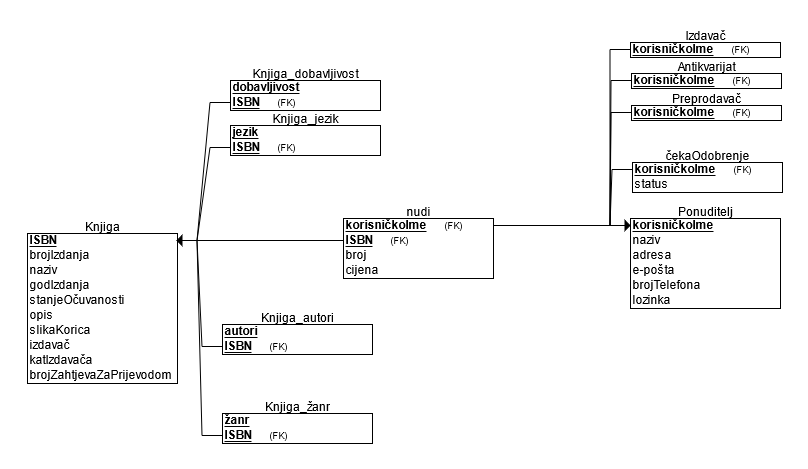
\includegraphics[width=\textwidth]{dijagrami/baza_relmod_v2.PNG} %veličina u odnosu na širinu linije
					\centering
					\caption{REL dijagram baze podataka}
					\label{fig:arh1}
				\end{figure}
				
				\eject
				
				\begin{figure}[H]
					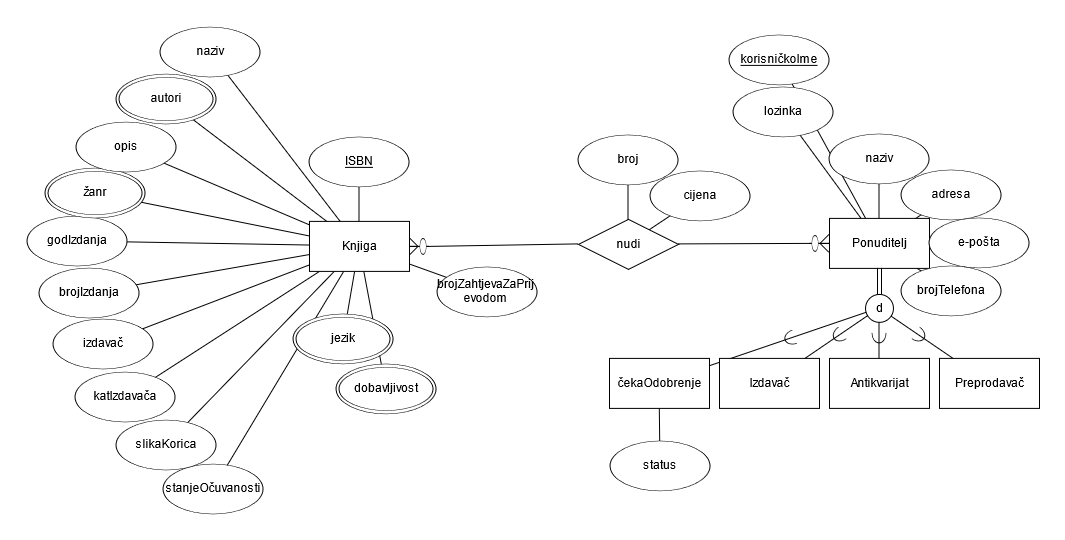
\includegraphics[width=\textwidth]{dijagrami/baza_ERmod_v2.PNG} %veličina u odnosu na širinu linije
					\centering
					\caption{ER dijagram baze podataka}
					\label{fig:arh2}
				\end{figure}
				
			
			\eject
			
			
		\section{Dijagram razreda}
		
			\textit{Potrebno je priložiti dijagram razreda s pripadajućim opisom. Zbog preglednosti je moguće dijagram razlomiti na više njih, ali moraju biti grupirani prema sličnim razinama apstrakcije i srodnim funkcionalnostima.}\\
			
			\textbf{\textit{dio 1. revizije}}\\
			
			\textit{Prilikom prve predaje projekta, potrebno je priložiti potpuno razrađen dijagram razreda vezan uz \textbf{generičku funkcionalnost} sustava. Ostale funkcionalnosti trebaju biti idejno razrađene u dijagramu sa sljedećim komponentama: nazivi razreda, nazivi metoda i vrste pristupa metodama (npr. javni, zaštićeni), nazivi atributa razreda, veze i odnosi između razreda.}\\
			
			\textbf{\textit{dio 2. revizije}}\\			
			
			\textit{Prilikom druge predaje projekta dijagram razreda i opisi moraju odgovarati stvarnom stanju implementacije}
			
			
			
			\eject
		
		\section{Dijagram stanja}
			
			
			\textbf{\textit{dio 2. revizije}}\\
			
			\textit{Potrebno je priložiti dijagram stanja i opisati ga. Dovoljan je jedan dijagram stanja koji prikazuje \textbf{značajan dio funkcionalnosti} sustava. Na primjer, stanja korisničkog sučelja i tijek korištenja neke ključne funkcionalnosti jesu značajan dio sustava, a registracija i prijava nisu. }
			
			
			\eject 
		
		\section{Dijagram aktivnosti}
			
			\textbf{\textit{dio 2. revizije}}\\
			
			 \textit{Potrebno je priložiti dijagram aktivnosti s pripadajućim opisom. Dijagram aktivnosti treba prikazivati značajan dio sustava.}
			
			\eject
		\section{Dijagram komponenti}
		
			\textbf{\textit{dio 2. revizije}}\\
		
			 \textit{Potrebno je priložiti dijagram komponenti s pripadajućim opisom. Dijagram komponenti treba prikazivati strukturu cijele aplikacije.}
